\section{0-1 knapsack problem}
This task describes the utilization of Particle Swarm Optimization algorithm utilized for solving so called Knapsack problem. In this task the amount of packages put inside the knapsack is only limited by the knapsack's weight limit.

It should be mentioned how the fitness function is represented. This specific implementation's aim is to minimize the value of fitness function which is expressed as the subtraction of the total value of all packages and the total value of packages present in the knapsack.

Figure \ref{fig:knaspack} shows the results of Particle Swarm Optimization algorithm used to solve the Knapsack problem with different values chosen for both local and global attraction coefficient. It can be seen that the algorithm gives the best result when both local and global attraction coefficients are set to the same value ($1.999$). If there is put focus either on local or global attraction the results are somewhat the same but worse as compared with the first case.

\begin{figure}[!h]
	\centering
		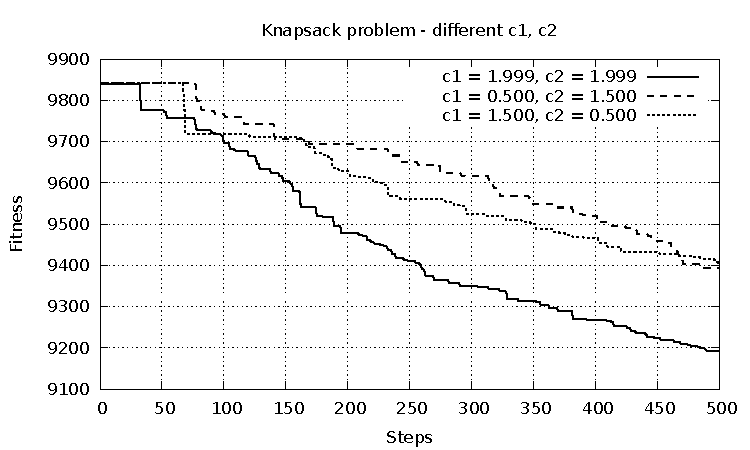
\includegraphics[width=15cm]{img/3b.pdf}
	\caption{Knapsack problem solution with different values for global and local attraction. The best result (full line) gained the fitness function value of 9191, while filling the knapsack up to 992.87 kg with total value of 722.4. The second best result (dashed line) gained the fitness function value of 9394, while filling the knapsack up to 997.56 kg with total value of 518.9. The worst result (dotted line) gained the fitness function value of 9406, while filling the knapsack up to 979.75 kg with total value of 506.9.}
	\label{fig:knaspack}
\end{figure}

Figure \ref{fig:knaspack} shows the results of Particle Swarm Optimization algorithm used to solve the Knapsack problem with different values chosen for both local and global attraction coefficient and with inertia support. It can be seen that no matter how many steps the result of the fitness function never changes. The reason might be the fact that due to the decreasing inertia and thus the decreasing velocity the particles are not able to search the wide are in search space and rather tend to return to their own best positions found.

\begin{figure}[!h]
	\centering
		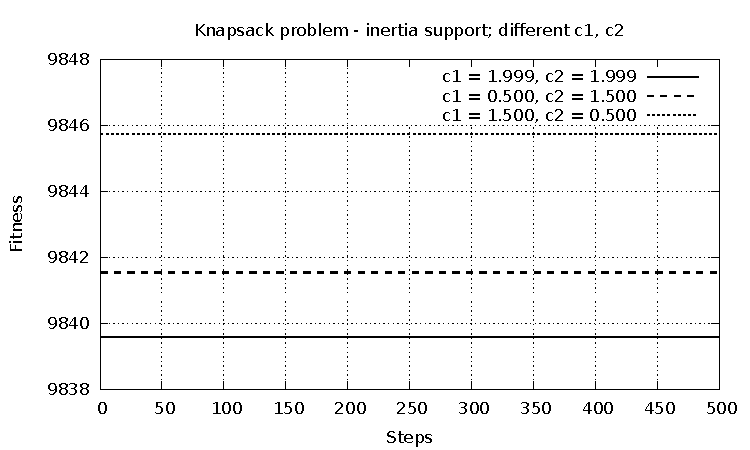
\includegraphics[width=15cm]{img/3c.pdf}
	\caption{Knapsack problem solution with different values for global and local attraction and support for inertia. Knapsack problem solution with different values for global and local attraction. The best result (full line) gained the fitness function value of 9840, while filling the knapsack up to 514.76 kg with total value of 73.9. The second best result (dashed line) gained the fitness function value of 9841, while filling the knapsack up to 578.9 kg with total value of 72.0. The worst result (dotted line) gained the fitness function value of 9846, while filling the knapsack up to 585.47 kg with total value of 67.76.}
	\label{fig:knaspack_inertia}
\end{figure}